\pdfminorversion=4
\documentclass[aspectratio=169]{beamer}
\usepackage{animate} % for animation
\usepackage{array,multirow,graphicx}
\usepackage{multicol}
\usepackage{etoolbox}
\graphicspath{{gambar/}}
\setbeamertemplate{caption}[numbered]
\setbeamertemplate{section in toc}[sections numbered]

% Hide subsubsections from TOC, but keep PDF bookmarks with beamer
\hypersetup{bookmarksopen=true,bookmarksopenlevel=4}
\setcounter{tocdepth}{4}

\renewcommand{\figurename}{Gambar.}
\renewcommand{\tablename}{Tabel.}

\usetheme[pageofpages=of,	% String used between the current page and the
							% total page count.
			alternativetitlepage=true,% Use the fancy title page.
			titleline=true,
			titlepagelogo=OK-LOGO-ITK.jpg
%          	 titlepagelogo=fig/jaist_logo.png
			]{Torino}
			% change /beamerinnerthemefancy.sty to resize the logo
\usecolortheme{freewilly}

\makeatletter
\patchcmd{\beamer@sectionintoc}{\vskip1.5em}{\vskip0em}{}{}
\makeatother

\author{Mifta Nur Farid, S.T., M.T. \\
	miftanurfarid@lecturer.itk.ac.id}
\title{RANGKAIAN ELEKTRONIKA II}
\subtitle{Penguat Operasional}
\institute{Teknik Elektro \\ Institut Teknologi Kalimantan \\ Balikpapan, Indonesia}
\date{\tiny Maret 8, 2021}

% The log drawn in the upper right corner.
\logo{
\includegraphics[height=0.13\paperheight]{OK-LOGO-ITK.jpg}}

\begin{document}

\begin{frame}[t,plain]
\titlepage
\end{frame}

%\begin{frame}{Bahan Kajian}
%	\begin{multicols}{2} % Two columns for outline
%    \tableofcontents[subsectionstyle=hide]
%	\end{multicols}
%\end{frame}

\section{Pengantar}
\begin{frame}{Pengantar}
\begin{figure}
	\centering
	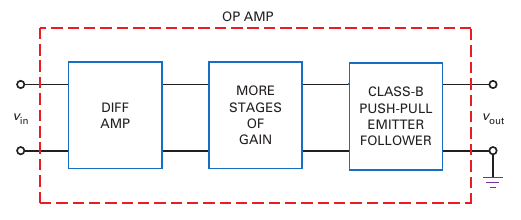
\includegraphics[width=0.7\linewidth]{gambar/fig-16.1}
	\caption{Blok diagram sebuah op amp}
	\label{fig:fig-16}
\end{figure}

\end{frame}
\section{Op Amp 741}
\begin{frame}{Op Amp 741}
	\begin{itemize}
		\item Item
	\end{itemize}
\end{frame}
\section{Inverting Amplifier}
\begin{frame}{Inverting Amplifier}
	\begin{itemize}
		\item Item
	\end{itemize}
\end{frame}
\section{Non-inverting Amplifier}
\begin{frame}{Non-inverting Amplifier}
	\begin{itemize}
		\item Item
	\end{itemize}
\end{frame}
\section{Aplikasi Op-Amp}
\begin{frame}{Aplikasi Op-Amp}
	\begin{itemize}
		\item Item
	\end{itemize}
\end{frame}
\begin{frame}
	\centering TERIMA KASIH
\end{frame}

\end{document}

